\documentclass[a4paper]{article}  

\usepackage[UTF8, scheme = plain]{ctex}
\usepackage{graphicx}
\usepackage{subfigure}
\usepackage{listings}
\usepackage{xcolor}
\usepackage{geometry}
\usepackage{amsmath}
\usepackage{float}

\geometry{a4paper,scale=0.8}

\graphicspath{ {images/} }

\lstset{
	basicstyle          =   \sffamily,          % 基本代码风格
	keywordstyle        =   \bfseries,          % 关键字风格
	commentstyle        =   \rmfamily\itshape,  % 注释的风格,斜体
	stringstyle         =   \ttfamily,  % 字符串风格
	flexiblecolumns,                % 别问为什么,加上这个
	numbers             =   left,   % 行号的位置在左边
	showspaces          =   false,  % 是否显示空格,显示了有点乱,所以不现实了
	numberstyle         =   \zihao{-5}\ttfamily,    % 行号的样式,小五号,tt等宽字体
	showstringspaces    =   false,
	captionpos          =   t,      % 这段代码的名字所呈现的位置,t指的是top上面
	frame               =   lrtb,   % 显示边框
}

\lstdefinestyle{CppStyle}{
	language        =   C++, 
	basicstyle      =   \zihao{-5}\ttfamily,
	numberstyle     =   \zihao{-5}\ttfamily,
	keywordstyle    =   \color{blue},
	keywordstyle    =   [2] \color{teal},
	stringstyle     =   \color{magenta},
	commentstyle    =   \color{red}\ttfamily,
	breaklines      =   true,   % 自动换行,建议不要写太长的行
	columns         =   fixed,  % 如果不加这一句,字间距就不固定,很丑,必须加
	basewidth       =   0.5em,
}

\renewcommand{\figurename}{图}
\renewcommand{\lstlistingname}{代码} 
\renewcommand{\tablename}{表格}
\renewcommand{\contentsname}{目录}

\title{实验七 \space 允许字符误差的KMP算法改进}
\author{熊恪峥 22920202204622}
\date{2021年12月17日}


\begin{document}
	\maketitle
	
	\tableofcontents 
	
	\newpage
	
	\section{允许一个字符误差的KMP算法}
	
	KMP一般认为有两种可能的实现,包括使用失配函数的实现和使用确定有限状态自动机(DFA, Deterministic finite automaton)的实现,它们的时间复杂度和空间复杂度基本相同,但DFA的实现有较大的常数。使用DFA的实现的匹配过程就是模拟DFA的运行过程,因而相当简单,易于进行修改。因此以下的改进基于\textit{Algorithms, 4th Edition}中的DFA实现的KMP算法。代码\ref{code:constructdfa}是该实现构建DFA的预处理过程。它用二维数组的方式存储DFA。
	
	\begin{lstlisting}[language=C++,numbers=left,style=CppStyle,caption=构建DFA的预处理代码,label={code:constructdfa}]
	static inline constexpr size_t PATTERN_LEN = 128;
	
	int dfa[CHAR_MAX][PATTERN_LEN]{};
	
	void construct(const std::string& pattern)
	{
		dfa[pattern.at(0)][0] = 1;
		for (int i = 1, x = 0; i < pattern.length(); i++)
		{
			for (char c = 0; c < CHAR_MAX; c++)
			{
				dfa[c][i] = dfa[c][x];
			}
			
			dfa[pattern.at(i)][i] = i + 1;
			x = dfa[pattern.at(i)][x];
		}
	}
	\end{lstlisting}

	例如对于模式串\textit{p='ababac'},构建出的DFA如图\ref{fig:dfa}。
	
	\begin{figure}[h]
		\caption{\textit{p='ababac'}的DFA}
		\centering
		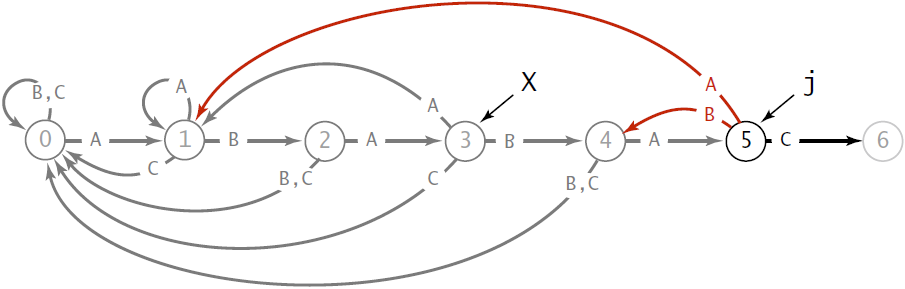
\includegraphics{dfa.png}
		
		\label{fig:dfa}
	\end{figure}

	从DFA的构造中容易知道,当失配时目标的状态值小于当前状态值。在这种情况首次发生时,如果跳过一个字符能够达到终止状态(情况1),或者能达到下一个匹配状态(情况二),就跳过一个字符,这样就能实现允许一个字符的误差。
	
	\begin{lstlisting}[language=C++,numbers=left,style=CppStyle,caption=允许一个错误的KMP匹配算法,label={code:allow1error}]
	int match(const std::string& pattern, const std::string& text, int pos)
	{
		int i = pos, j = 0;
		
		bool e = false;
		for (; i < text.length() && j < pattern.length(); i++)
		{
			//情况一
			if (dfa[text.at(i)][j] <= j && j == pattern.length() - 1)
			{
				e = true;
				j++;
				i++;
				break;
			}
			//情况二
			else if (dfa[text.at(i)][j] <= j && i + 1 < text.length() && j + 1 < pattern.length() &&
			text.at(i + 1) == pattern.at(j + 1) && !e)
			{
				e = true;
				j++;
			}
			else
			{
				j = dfa[text.at(i)][j];
			}
		}
		
		if (j == pattern.length())
		{
			return i - pattern.length();
		}
		
		return text.length();
	}
	\end{lstlisting}

	\subsection{该改进算法的正确性}
	
	\begin{enumerate}
		\item 当主串$T$中没有和模式串$p$中差一个字符匹配的子串时,该算法和使用DFA的KMP实现相同,因此是正确的。
		\item 当主串$T$中存在和模式串$p$中差一个字符匹配的子串时,遇到该失配字符前该算法的行为与和使用DFA的KMP实现相同,跳过一个适配字符之后该算法的行为也和使用DFA的KMP实现相同,因此是正确的。
	\end{enumerate}

	或者可以从DFA图出发论证该改进的正确性,该改进相当于在每两个状态之间添加一个转移,转移的条件是已经跳过的字符数量小于1个。那么原始的DFA是新的DFA的一个子图,因此它不影响正常的字符匹配。由新加的转移的条件可以知道,它允许有一个误差的输入到达终止状态。因此它的正确性是显然的。

	实际测试表明该代码确实能正确完成允许一个失配字符的模式匹配功能。
	
	\subsection{改进算法的时间复杂度}
	该算法的预处理过程与使用DFA的KMP的预处理过程实现相同,是$O(MR)$,其中$R$是字母表的长度,是一个常数。而匹配过程最多比普通的KMP多出一次比较,因此时间复杂度亦没有改变。

	\section{允许多个字符误差的KMP算法}
	
	使用相同的思路可以将该算法扩展成允许多个字符误差的匹配算法,代码\ref{code:allowmanyerror}中匹配函数的参数$e\_allow$控制允许多少个字符的误差。它在发生失配时会试图检查跳过不超过$e\_allow$个字符能否到达终止状态或者一个匹配状态。

	\begin{lstlisting}[language=C++,numbers=left,style=CppStyle,caption=允许指定错误数量的KMP匹配算法,label={code:allowmanyerror}]
	int match(const std::string& pattern, const std::string& text, int pos, int e_allow)
	{
		int i = pos, j = 0;
		
		int e = 0;
		for (; i < text.length() && j < pattern.length(); i++)
		{
			if (dfa[text.at(i)][j] <= j && e < e_allow)
			{
				
				int e_cnt = 0, ni = i, nj = j;
				while (ni < text.length() && nj < pattern.length() && text.at(ni) != pattern.at(nj) && e_cnt < e_allow)
				{
					ni++;
					nj++;
					e_cnt++;
				}
				
				if (ni < text.length() && nj < pattern.length() && text.at(ni) == pattern.at(nj))
				{
					i = ni - 1;
					j = nj;
					e = e_cnt;
				}
				else if (nj == pattern.length())
				{
					i = ni;
					j = nj;
					e = e_cnt;
					break;
				}
				else
				{
					j = dfa[text.at(i)][j];
				}
			}
			else
			{
				j = dfa[text.at(i)][j];
			}
		}
		
		if (j == pattern.length())
		{
			return i - pattern.length();
		}
		
		return text.length();
	}
	
	\end{lstlisting}

	该算法的正确性说明同上,但时间复杂度并不与普通的KMP实现相同,它与要允许的错误数量$E$和主串$T$中存在的符合条件的字串数量有关。

\end{document}